\documentclass{beamer}
\usepackage{tikz} %for mindmap
\usetikzlibrary{mindmap} %for mindmap
\usepackage{pgfpages}
\usepackage[backend=bibtex]{biblatex}
\usepackage{multicol}
\usepackage{textpos}
\setbeameroption{hide notes} % Only slides
%\setbeameroption{show only notes} % Only notes
%\setbeameroption{show notes on second screen=right} % Both
\bibliography{../../papers/references.bib}
\setbeamerfont{footnote}{size=\small}
%\AtEveryCitekey{\clearfield{title}}
\expandafter\def\expandafter\insertshorttitle\expandafter{%
   \insertshorttitle\hfill%
   \insertframenumber\,/\,\inserttotalframenumber}

%
% Choose how your presentation looks.
%
% For more themes, color themes and font themes, see:
% http://deic.uab.es/~iblanes/beamer_gallery/index_by_theme.html
%
\mode<presentation>
{
   \usetheme{Warsaw}      % or try Darmstadt, Madrid, Warsaw, ...
   \usecolortheme{default} % or try albatross, beaver, crane, ...
   \usefonttheme{default}  % or try serif, structurebold, ...
   \setbeamertemplate{navigation symbols}{}
%   \setbeamertemplate{caption}[numbered]
%   \setbeamertemplate{footline}[frame number]
   \usepackage{appendixnumberbeamer} %starts slide numbering over after \appendix
} 

\usepackage[english]{babel}
%\usepackage[utf8x]{inputenc} %Doesn't play well with biblatex
\usepackage{amssymb}
\usepackage{bm}
\usepackage{color}
\usepackage{graphicx}

\newcommand{\red}[1]{{\color{red}{#1}}}
\newcommand{\blue}[1]{{\color{blue}{#1}}}
\newcommand{\ket}[1]{\left| #1 \right>}
\newcommand{\bra}[1]{\left< #1 \right|}
\newcommand{\braket}[2]{\left< #1 | #2 \right>}
\newcommand{\ketbra}[2]{\left| #1 \right> \left< #2 \right|}
\newcommand{\expect}[1]{\left< #1 \right>}
\newcommand{\fpij}{f_p(r_{ij})}
\newcommand{\vpij}{v_p(r_{ij})}
\newcommand{\Opij}{\mathcal{O}_{ij}^p}
\newcommand{\fOpij}{\sum\limits_{i<j}\sum\limits_p \fpij\Opij}
\newcommand{\fqkl}{f_q(r_{kl})}
\newcommand{\Oqkl}{\mathcal{O}_{kl}^q}
\newcommand{\fOqkl}{\sum\limits_{k<l}\sum\limits_q \fqkl\Oqkl}
\newcommand{\fOqklip}{\sum\limits_{k<l,\mathrm{ip}}\sum\limits_q \fqkl\Oqkl}
\newcommand{\fOqklquad}{\sum_{\substack{k<l\\ij \ne kl}}\sum\limits_q \fqkl\Oqkl}
\newcommand{\f}[2]{f_{#1}(r_{#2})}
\renewcommand{\O}[2]{\mathcal{O}_{#2}^{#1}}
\newcommand{\fO}[2]{\sum\limits_{#1} f_{#1}(r_{#2})\mathcal{O}_{#2}^{#1}}
\newcommand{\R}{\mathbf{R}}
\renewcommand{\r}{\mathbf{r}}
\newcommand{\dt}{\Delta\tau}
\newcommand{\ti}{\bm{\tau}_i}
\newcommand{\tj}{\bm{\tau}_j}
\newcommand{\si}{\bm{\sigma}_i}
\newcommand{\sj}{\bm{\sigma}_j}
\newcommand{\sfont}{6}
\newcommand{\sspace}{10.2}
\newcommand{\Oijp}{\mathcal{O}^p_{ij}}

\title[Nuclear QMC]{Nuclear Quantum Monte Carlo at SUU}
\author[Cody L. Petrie, cody.petrie@asu.edu]{Cody L. Petrie}
\institute{Southern Utah University \\ Cedar City, UT}
\date{}

\begin{document}

\begin{frame}
   \titlepage
%   \centering
%   \vspace{-1.0cm}
%   \small
%Collaborators: Stefano Gandolfi (LANL), Joe Carlson (LANL) \\~\\
%INT Program INT-18-2b Advances in Monte Carlo Techniques for Many-Body Quantum Systems \\
%July 30 - September 7, 2018
\end{frame}

\begin{frame}{Outline}
\begin{itemize}
   \item What problems I work on + background
   \item Method I use to solve problems
   \item Specific work I've done
   \item Results I've gotten
   \item Future work/Conclusion
\end{itemize}
\end{frame}

\begin{frame}{Questions}
\begin{center}
   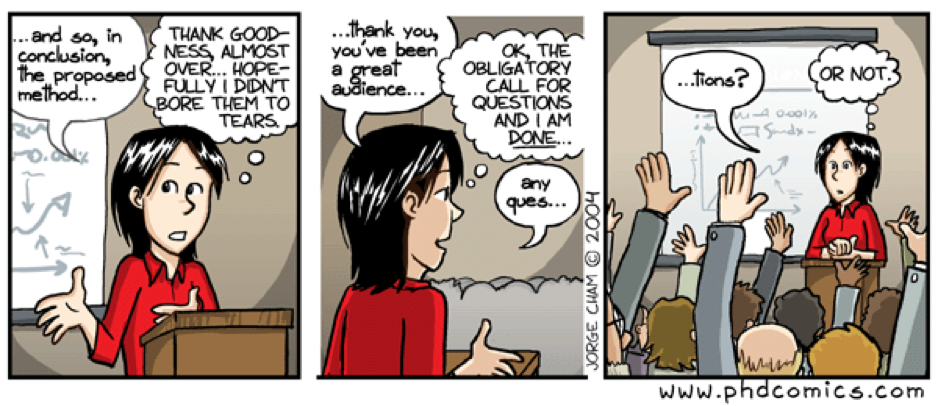
\includegraphics[width=1.0\textwidth]{figures/questions_comic.png}
\end{center}
\end{frame}

\begin{frame}[t]{Why Nuclear Physics?}
\begin{itemize}
   \item Nuclear physics has been an important topic to study for over a century
   \begin{itemize}
      \item Nuclear energy
      \item Radiotherapy to kill cancer cells
      \item Nuclear Magnetic Resonance (MRI imaging)
      \item Radioactive dating
   \end{itemize}
   to name a few \ldots
\end{itemize}
\begin{textblock*}{\textwidth}(2.8cm,0.15cm) % {block width} (coords)
   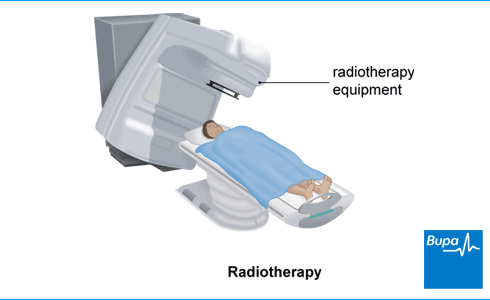
\includegraphics[width=4.0cm]{figures/radiotherapy.png}
\end{textblock*}
\begin{textblock*}{\textwidth}(-0.5cm,1.5cm) % {block width} (coords)
   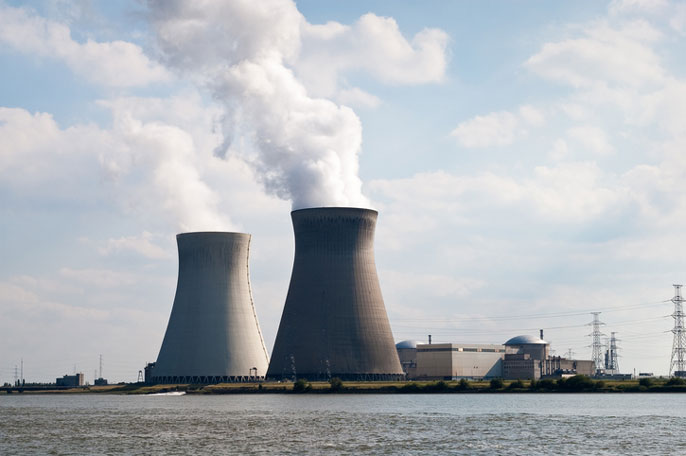
\includegraphics[width=4.0cm]{figures/nuclear_energy.jpg}
\end{textblock*}
\begin{textblock*}{\textwidth}(7.3cm,-0.8cm) % {block width} (coords)
   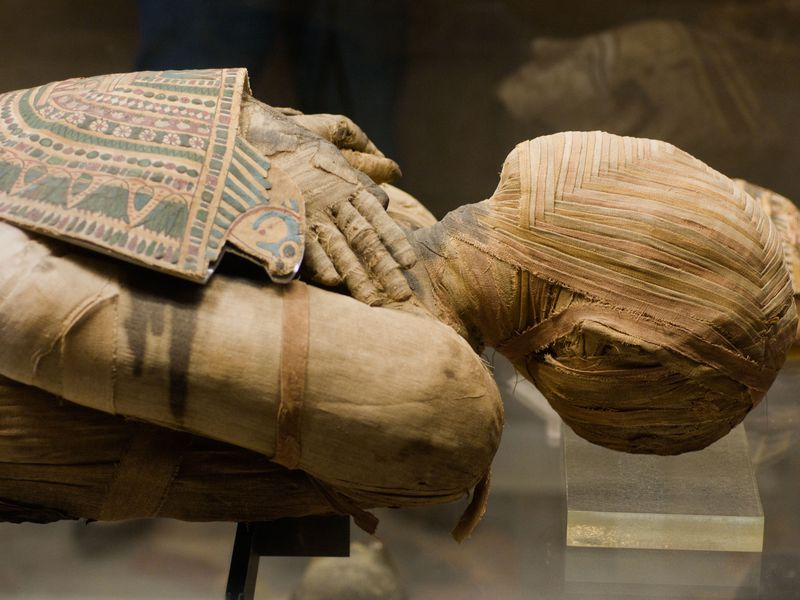
\includegraphics[width=4.0cm]{figures/mummy.jpg}
\end{textblock*}
\begin{textblock*}{\textwidth}(6.0cm,1.6cm) % {block width} (coords)
   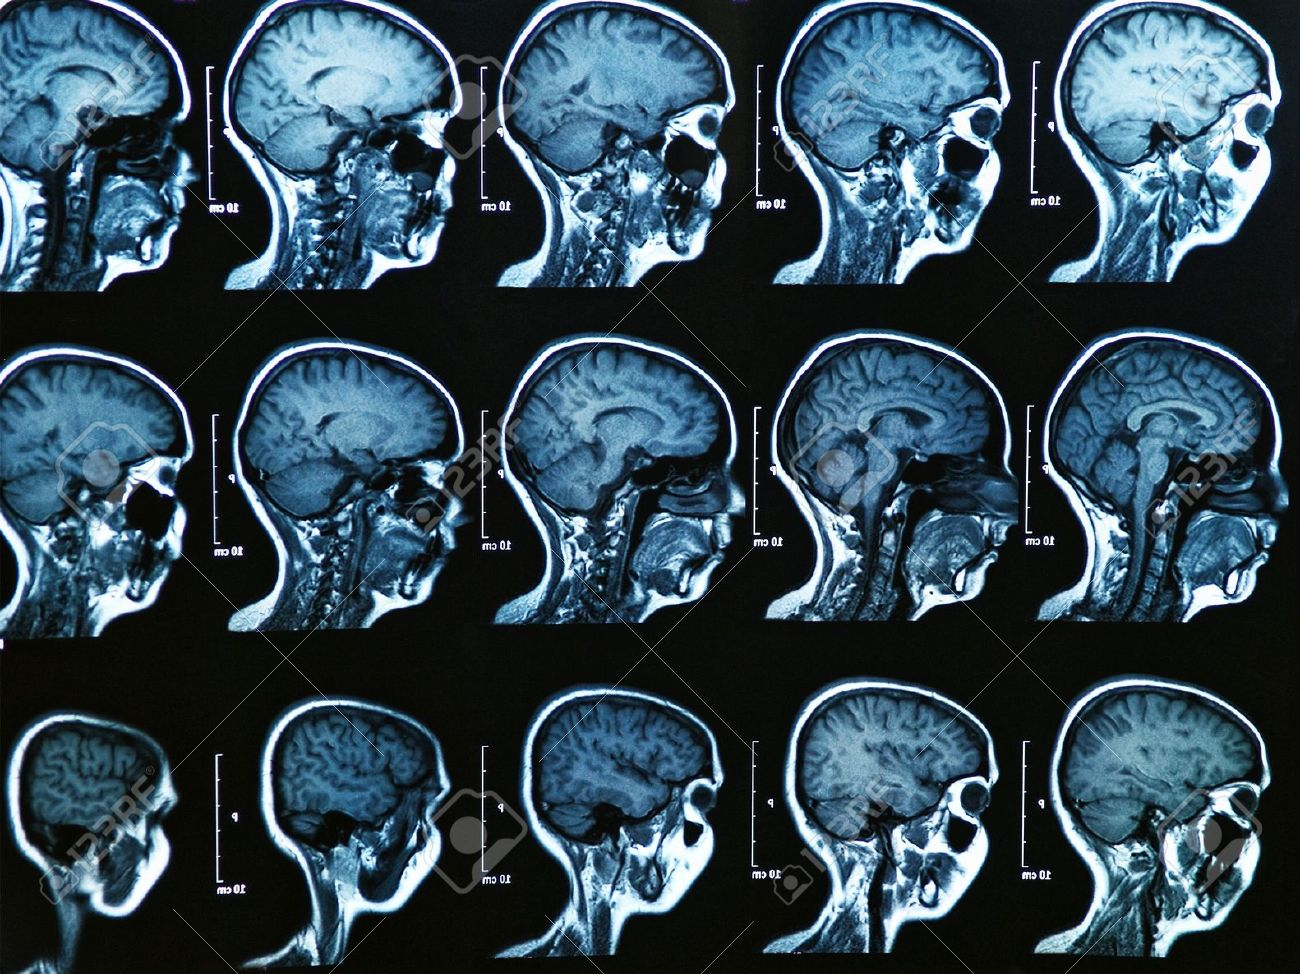
\includegraphics[width=4.0cm]{figures/mri.jpg}
\end{textblock*}
\end{frame}

\begin{frame}{Why Nuclear Physics?}
\begin{itemize}
   \item Much of this was done without a good understanding of how nuclear particles interact with each other.
   \item My research has to do with understanding that fundamental interaction between nuclear particles (called nucleons).
\end{itemize}
\begin{center}
   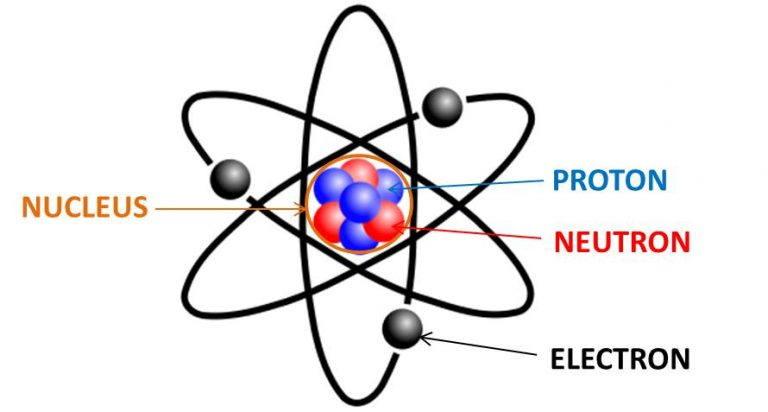
\includegraphics[width=0.6\textwidth]{figures/atom.jpg}
\end{center}
\end{frame}

\begin{frame}{Nuclear Problem}
\begin{itemize}
   \item We want to solve for the ground state energy of nuclei. This is also called the {\bf binding energy}, $B$.
   \begin{equation*}
      B = Zm_pc^2 + Nm_nc^2 - m_\text{nuclei}c^2
   \end{equation*}
   \item<2-> Quantum Mechanics tells us that this energy is equal to
   \begin{equation*}
      E_0 = -B = \int d\r_1\ldots d\r_A \Psi_0^*(\r_1,\ldots,\r_A) \hat{H} \Psi_0(\r_1,\ldots,\r_A)
   \end{equation*}
   But let's break this down a bit.
\end{itemize}
\end{frame}

\begin{frame}{Nuclear Problem}
\begin{equation*}
   E_0 = \int d\r_1\ldots d\r_A \Psi_0^*(\r_1,\ldots,\r_A) \hat{H} \Psi_0(\r_1,\ldots,\r_A)
\end{equation*}
\begin{itemize}
   \item $d\r_i = dx_idy_idz_i$ so really it's a $3A$ dimensional integral.
   \item<2-> $\hat{H}$ is called the Hamiltonian. This is just a fancy way of saying the thing that tells us what the energy is. For the EM force it's something like
   \begin{equation*}
      H_\text{EM} = \sum\limits_{i=1}^N \frac{p_i^2}{2m} + \sum\limits_{i<j} k\frac{q_1q_2}{r_{ij}}
   \end{equation*}
   \item<3-> The last part, $\Psi_0$,  is called the wave function, and it deserves it's own slide.
\end{itemize}
\end{frame}

\begin{frame}{Wave Function}
\begin{itemize}
   \item Ingredients to describe the state of a classical system:
   \begin{itemize}
      \item Position and momentum (velocity) of each particle.
   \end{itemize}
   \item If we knew those things for every particle we could (classically) predict everything in the universe.
\end{itemize}
\begin{center}
   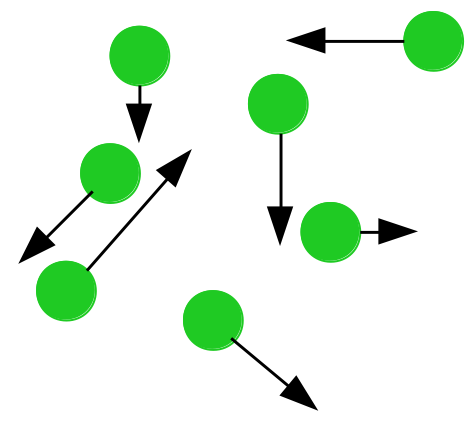
\includegraphics[width=0.5\textwidth]{figures/pos_vel.png}
\end{center}
\end{frame}

\begin{frame}{Wave Function}
\begin{itemize}
   \item Quantum Mechanics tells us that particles don't have just a single position, but they can be in multiple places at the same time. The probability of finding a particle in a given place is given by the square of the {\bf wave function}, $\left|\Psi(\R)\right|^2$.
   \item You've probably seen this idea before:
\end{itemize}
\begin{center}
   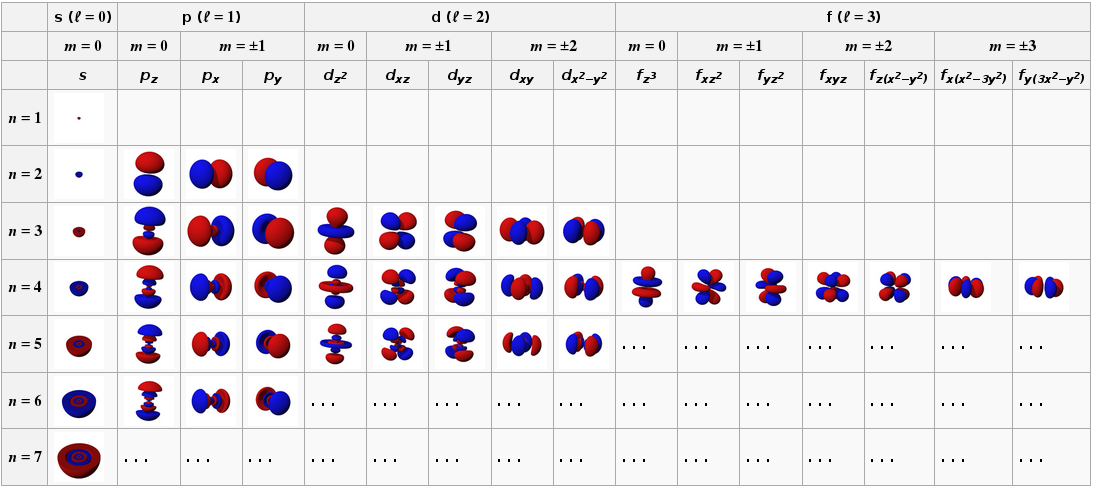
\includegraphics[width=1.0\textwidth]{figures/ylm_orbitals.png}
\end{center}
\end{frame}

\begin{frame}{Wave Functions}
\begin{itemize}
   \item The state that has the lowest energy is called the {\bf ground state}.
   \item All we need to do now is plug in the ground state $\Psi_0(\r_1,\ldots,\r_A)$, the nuclear Hamiltonian $\hat{H}$, and solve the integral\ldots that's it!
\end{itemize}
\begin{equation*}
   E_0 = \int d\r_1\ldots d\r_A \Psi_0^*(\r_1,\ldots,\r_A) \hat{H} \Psi_0(\r_1,\ldots,\r_A)
\end{equation*}
\begin{itemize}
   \item<2-> There are only a couple of small problems:
   \begin{itemize}
      \item<3-> We don't actually know a great way to write $\hat{H}$ for nuclear physics.
      \item<4-> We don't know what the ground state is.
      \item<5-> The integrals are too big and complicated for our computers to solve using normal numerical integration methods.
   \end{itemize}
\end{itemize}
\end{frame}

\begin{frame}{Solving the Problems - $\hat{H}$}
\begin{itemize}
   \item Two methods we use to get approximations to $\hat{H}$:
   \begin{itemize}
      \item {\bf Phenomenological Approach:} Make an educated guess and then smash particles together and fit the guess to the data.
         \begin{center}
            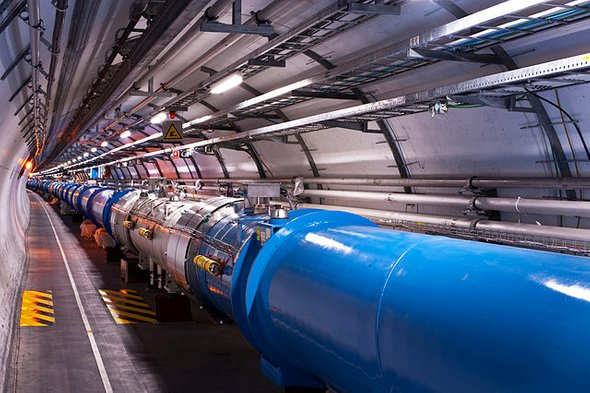
\includegraphics[width=0.4\textwidth]{figures/lhc.jpg}
         \end{center}
      \item {\bf Quantum Field Theory Approach:} Make approximations to the ``true" theory to determine what the interaction will look like.
         \begin{center}
            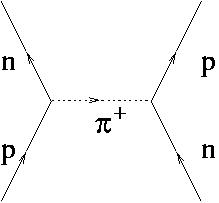
\includegraphics[width=0.2\textwidth]{figures/pion_exchange.jpg}
         \end{center}
   \end{itemize}
\end{itemize}
\end{frame}

\begin{frame}{Solving the Problems - $\Psi_0(\r_1,\ldots,\r_A)$}
\begin{itemize}
   \item One guess for the wave function would be to find ``single particle" states and put each particle in one of those;
   \begin{equation*}
      \Psi_0(\r_1,\ldots,\r_A) = \phi_1(\r_1)\phi_2(\r_2)\ldots\phi_A(\r_A)\footnotemark
   \end{equation*}
   \item<2-> This is a good start but notice that the particles don't interact in this wave function. Let's force this in.
   \begin{equation*}
      \Psi_0(\r_1,\ldots,\r_A) = \left[1+\sum\limits_{i<j}\mathcal{O}_{ij}\right]\Phi(\r_1,\ldots,\r_A)
   \end{equation*}
\begin{figure}[h]
\newcommand\shift{2.2}
\newcommand\vshift{-1.5} %vertical shift
\newcommand\tshift{0.05} %tiny shift
\newcommand\sep{0.75}
   \centering
   \begin{tikzpicture}[>=latex,scale=1.0]
      \filldraw[black] (0*\shift,0)          circle (2pt) node[anchor=east] {\large 1};
      \filldraw[black] (0*\shift,\sep)       circle (2pt) node[anchor=east] {\large 2};
      \filldraw[black] (0*\shift+\sep,0)     circle (2pt) node[anchor=west] {\large 3};
      \filldraw[black] (0*\shift+\sep,\sep)  circle (2pt) node[anchor=west] {\large 4};
      \draw[black, ultra thick] (0*\shift,\sep) -- (0*\shift,0); %i-j

      \filldraw[black] (1*\shift,0)          circle (2pt) node[anchor=east] {\large 1};
      \filldraw[black] (1*\shift,\sep)       circle (2pt) node[anchor=east] {\large 2};
      \filldraw[black] (1*\shift+\sep,0)     circle (2pt) node[anchor=west] {\large 3};
      \filldraw[black] (1*\shift+\sep,\sep)  circle (2pt) node[anchor=west] {\large 4};
      \draw[black, ultra thick] (1*\shift,0) -- (1*\shift+\sep,0); %k-l

      \filldraw[black] (2*\shift,0)          circle (2pt) node[anchor=east] {\large 1};
      \filldraw[black] (2*\shift,\sep)       circle (2pt) node[anchor=east] {\large 2};
      \filldraw[black] (2*\shift+\sep,0)     circle (2pt) node[anchor=west] {\large 3};
      \filldraw[black] (2*\shift+\sep,\sep)  circle (2pt) node[anchor=west] {\large 4};
      \draw[black, ultra thick] (2*\shift+\sep,\sep) -- (2*\shift,0); %k-l

      \filldraw[black] (0*\shift,\vshift)             circle (2pt) node[anchor=east] {\large 1};
      \filldraw[black] (0*\shift,\sep+\vshift)        circle (2pt) node[anchor=east] {\large 2};  
      \filldraw[black] (0*\shift+\sep,\vshift)        circle (2pt) node[anchor=west] {\large 3}; 
      \filldraw[black] (0*\shift+\sep,\sep+\vshift)   circle (2pt) node[anchor=west] {\large 4};
      \draw[black, ultra thick] (0*\shift,\sep+\vshift) -- (0*\shift+\sep,\vshift); %i-j

      \filldraw[black] (1*\shift,\vshift)       circle (2pt) node[anchor=east] {\large 1};
      \filldraw[black] (1*\shift,\sep+\vshift)  circle (2pt) node[anchor=east] {\large 2};
      \filldraw[black] (1*\shift+\sep,\vshift)  circle (2pt) node[anchor=west] {\large 3};  
      \filldraw[black] (1*\shift+\sep,\sep+\vshift) circle (2pt) node[anchor=west] {\large 4};
      \draw[black, ultra thick] (1*\shift,\sep+\vshift) -- (1*\shift+\sep,\sep+\vshift); %i-j

      \filldraw[black] (2*\shift,\vshift)             circle (2pt) node[anchor=east] {\large 1};  
      \filldraw[black] (2*\shift,\sep+\vshift)        circle (2pt) node[anchor=east] {\large 2};  
      \filldraw[black] (2*\shift+\sep,\vshift)        circle (2pt) node[anchor=west] {\large 3};
      \filldraw[black] (2*\shift+\sep,\sep+\vshift)   circle (2pt) node[anchor=west] {\large 4};
      \draw[black, ultra thick] (2*\shift+\sep,\vshift) -- (2*\shift+\sep,\sep+\vshift); %i-j
   \end{tikzpicture}
\end{figure}
\end{itemize}
\footnotetext[1]{We technically antisymmetrize this with respect to particle exchange.}
\end{frame}

\begin{frame}{Solve the Problems - Monte Carlo Integration}
\begin{center}
   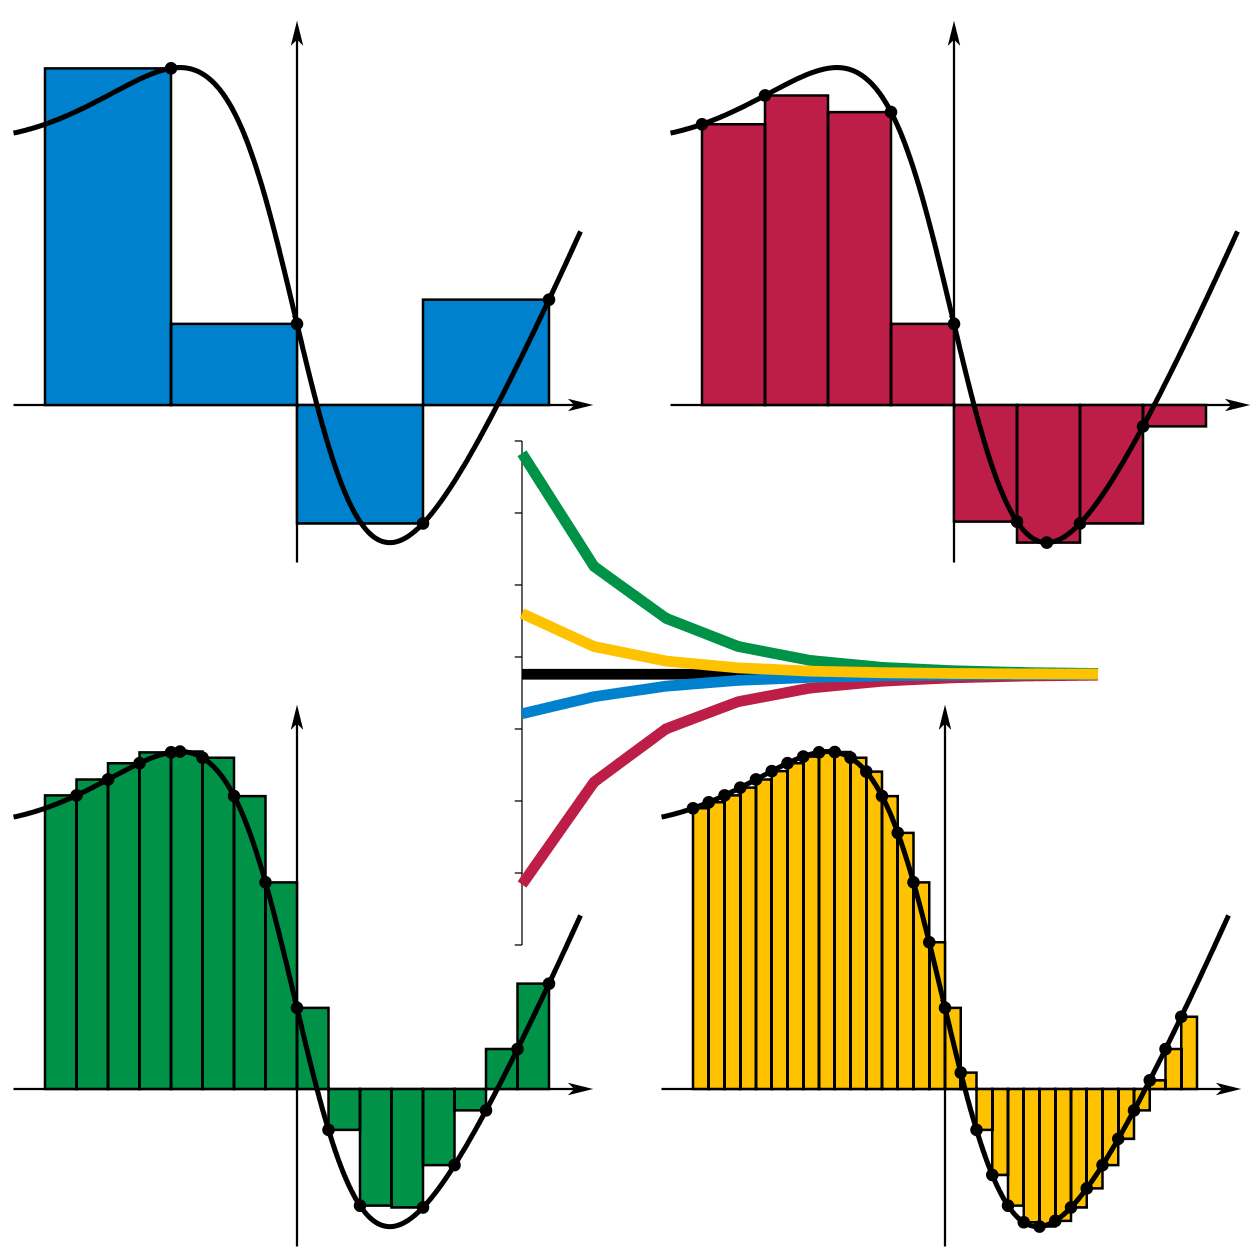
\includegraphics[width=0.5\textwidth]{figures/riemann_sum.png}
\end{center}
\begin{itemize}
   \item At 1000 samples per dimension that's $10^{15}$, $10^{51}$, and $10^{123}$ samples just to calculate the intergral for $^4$He, $^{16}$O, and $^{40}$Ca respectively. 
   \item That's infeasible! We need something else.
\end{itemize}
\end{frame}

\begin{frame}{Solve the Problems - Monte Carlo Integration}
\begin{itemize}
   \item Let's try the Monte Carlo method. Monte Carlo uses random samples instead of a defined number of grid points. Let's integrate to find the area of a circle.
\end{itemize}
\onslide<1>{
\begin{textblock*}{\textwidth}(2.5cm,-0.3cm) % {block width} (coords)
\begin{figure}[h]
   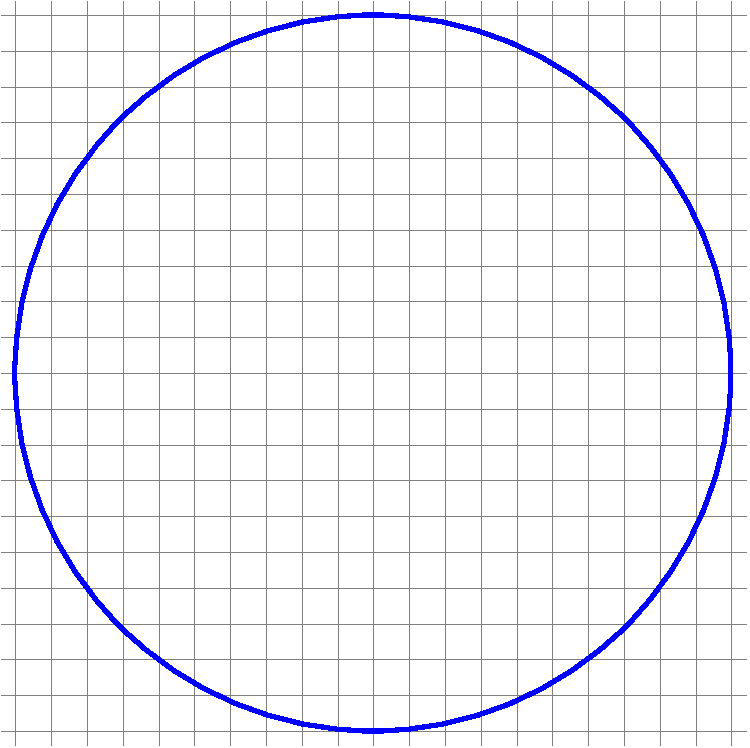
\includegraphics[width=0.4\textwidth]{figures/circle_grid.pdf}
\end{figure}
\end{textblock*}
}
\only<1>{
\vspace{5.5cm}
\begin{equation*}
   A_\text{circle} = \sum\limits_{i}\sum\limits_{j} dx_i dy_j
\end{equation*}
}
\onslide<2>{
\begin{textblock*}{\textwidth}(-3.3cm,1.0cm) % {block width} (coords)
\begin{figure}[h]
   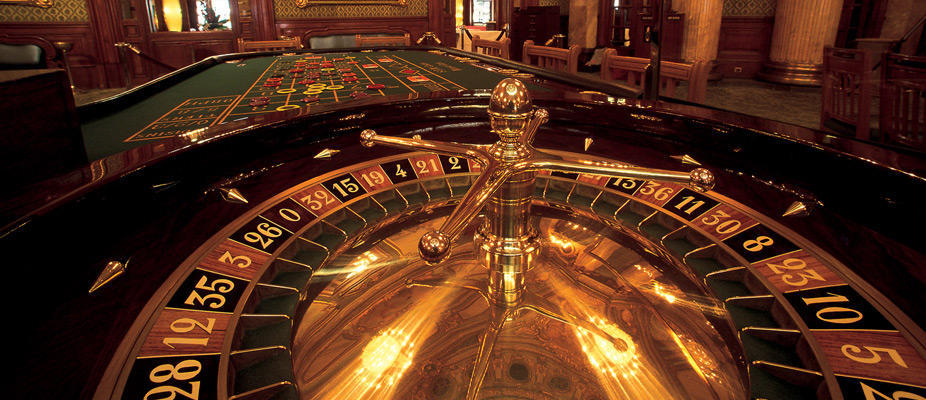
\includegraphics[width=0.4\textwidth]{figures/monte_carlo_casino.jpg}
\end{figure}
\end{textblock*}
\begin{textblock*}{\textwidth}(2.5cm,-0.3cm) % {block width} (coords)
\begin{figure}[h]
   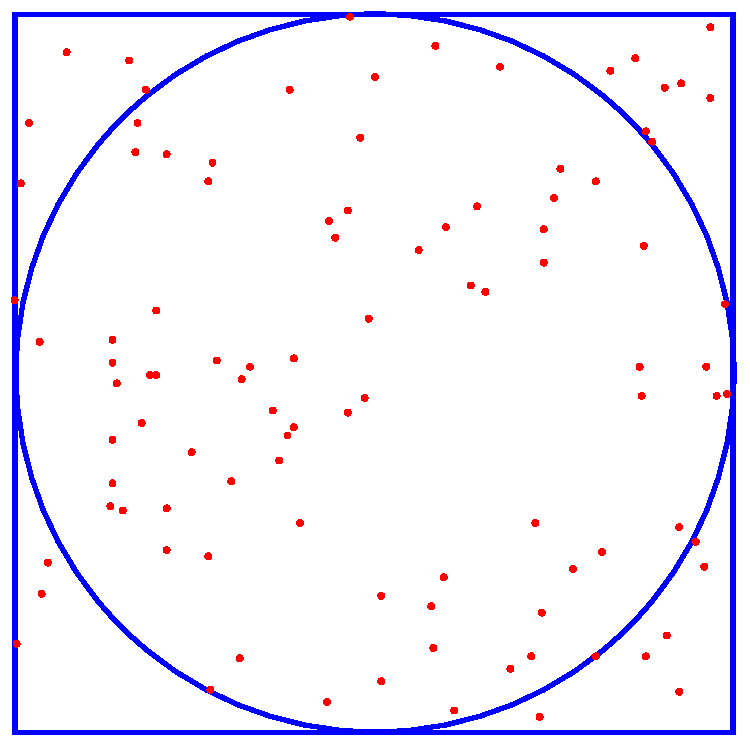
\includegraphics[width=0.4\textwidth]{figures/circle_square_points.pdf}
\end{figure}
\end{textblock*}
}
\vspace{5.5cm}
\only<2>{
\begin{equation*}
   \frac{A_\text{circle}}{A_\text{box}} = \frac{\text{\# points in the circle}}{\text{\# points in the box (total)}}
\end{equation*}
}
\end{frame}

\begin{frame}{Monte Carlo Example}
\begin{itemize}
   \item You can estimate $\pi=3.14159$ using the method above.
\begin{equation*}
   \frac{A_\text{circle}}{A_\text{box}} = \frac{\pi r^2}{(2r)(2r)} = \frac{\pi}{4} = \frac{\text{\# points in the circle}}{\text{\# points in the box (total)}}
\end{equation*}
\begin{equation*}
   \pi=4\frac{\text{\# points in the circle}}{\text{\# points in the box (total)}}
\end{equation*}
\end{itemize}
\begin{figure}[h]
   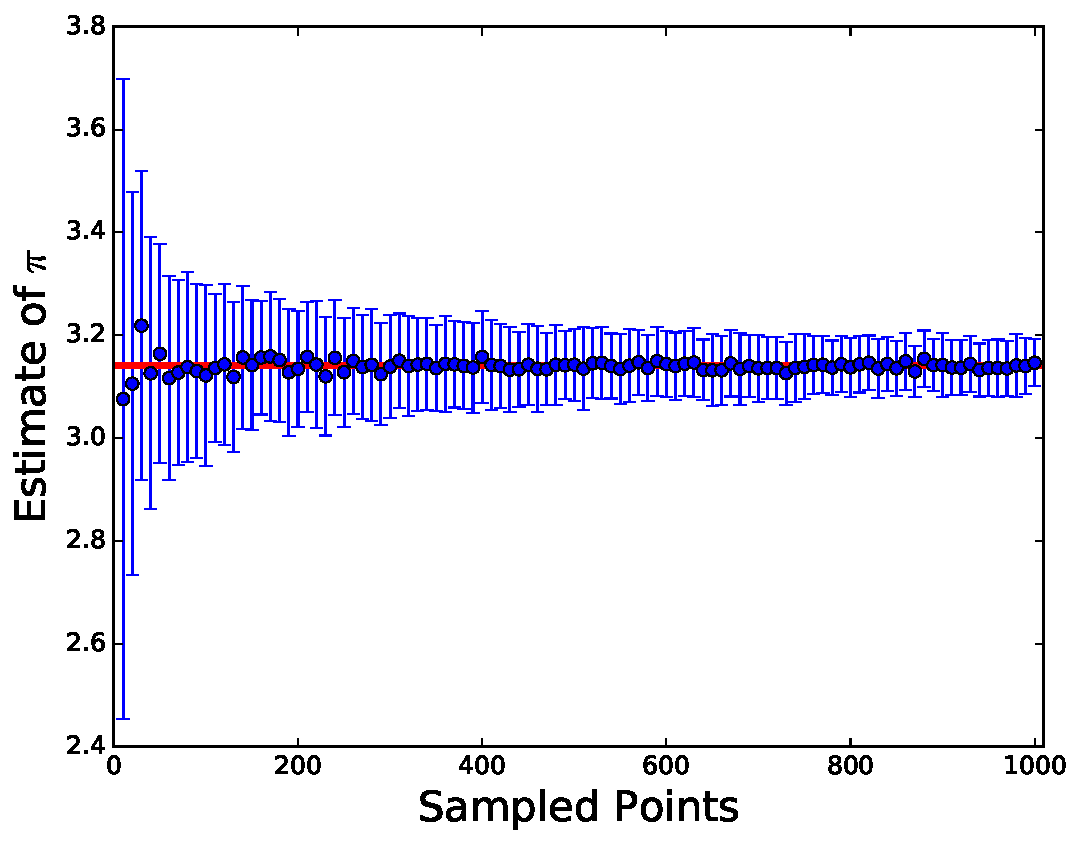
\includegraphics[width=0.55\textwidth]{figures/pi_estimate.pdf}
\end{figure}
\end{frame}

\begin{frame}{Monte Carlo on a Supercomputer}
\begin{textblock*}{\textwidth}(-3.6cm,0.0cm) % {block width} (coords)
\begin{figure}[h]
   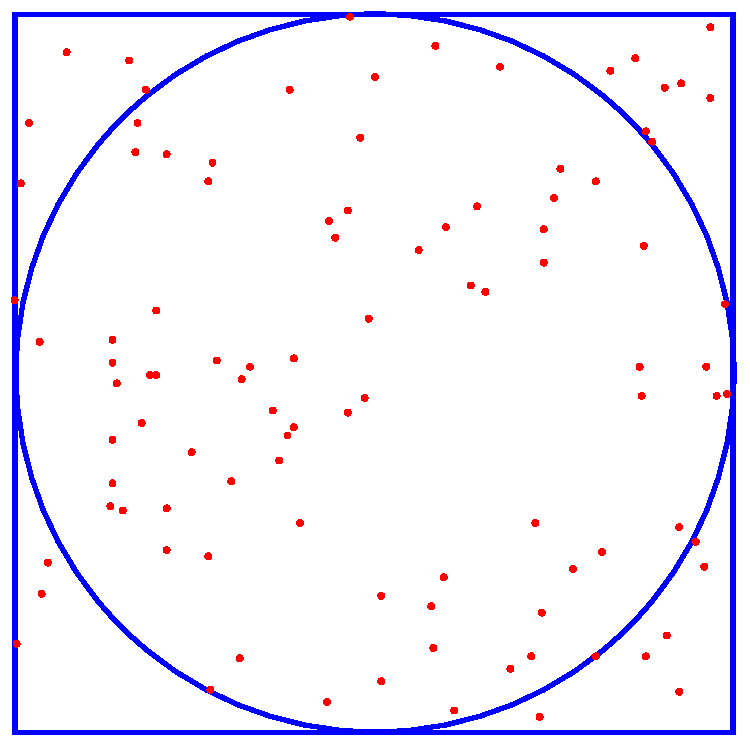
\includegraphics[width=0.3\textwidth]{figures/circle_square_points.pdf}
\end{figure}
\end{textblock*}
\begin{textblock*}{\textwidth}(2.2cm,-0.5cm) % {block width} (coords)
\begin{figure}[h]
   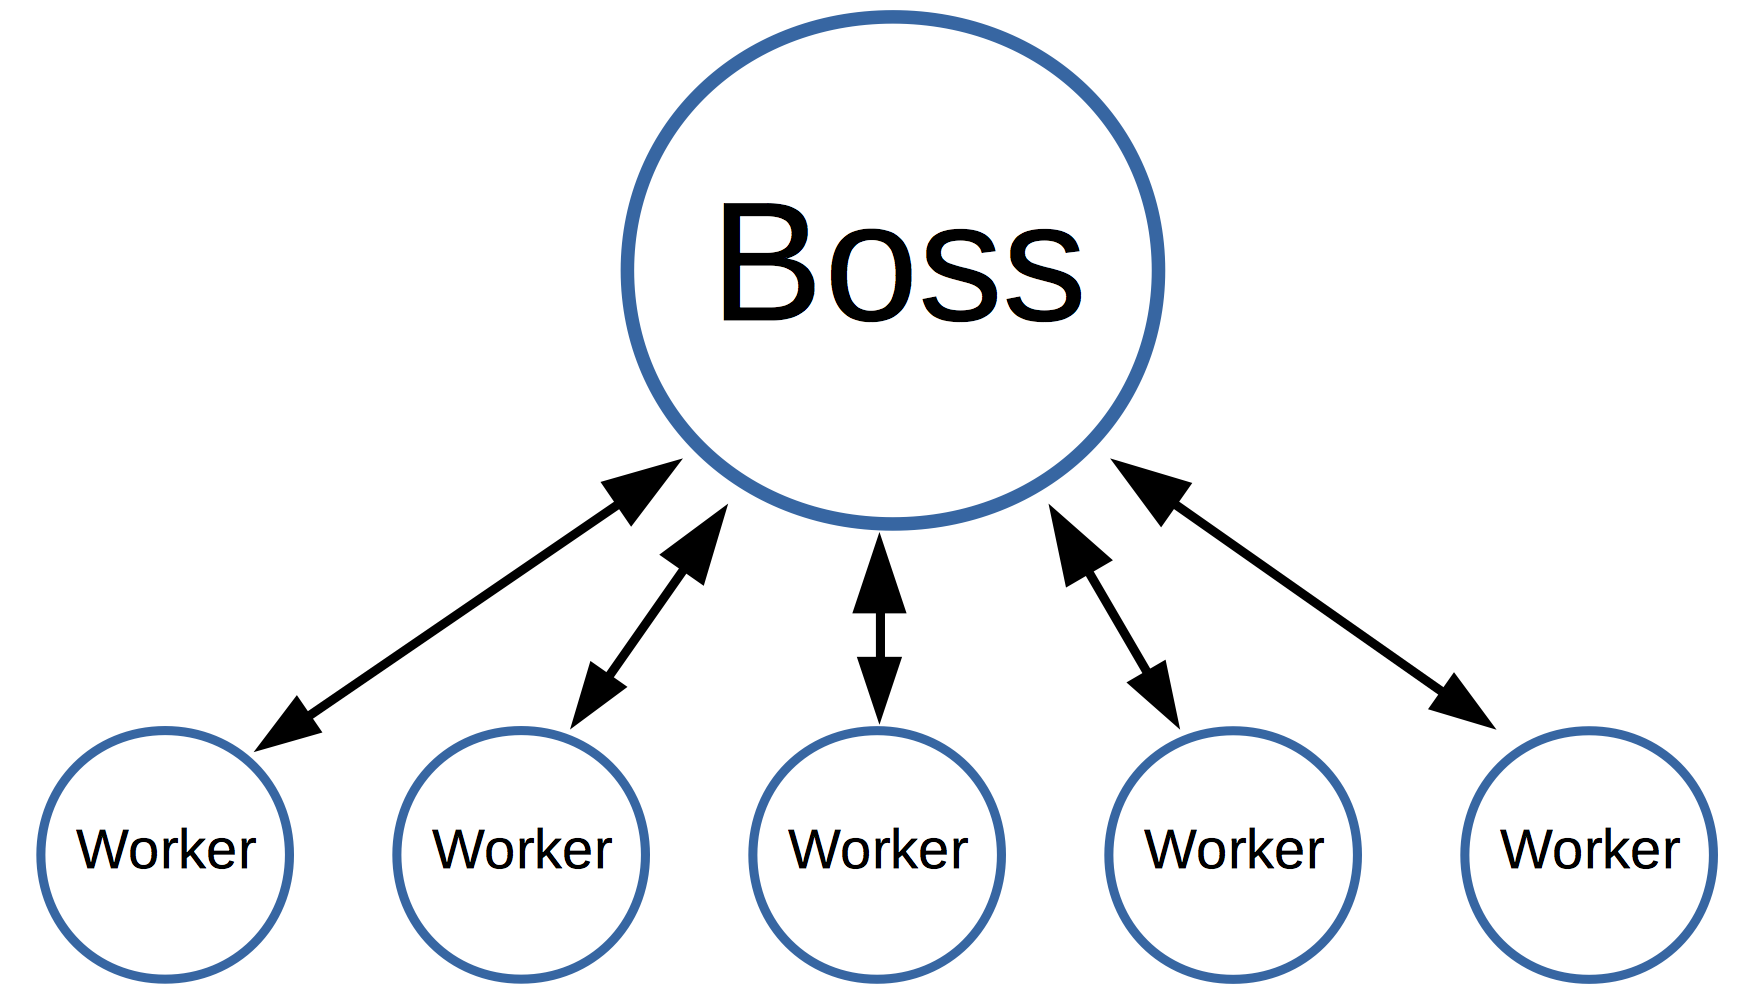
\includegraphics[width=0.7\textwidth]{figures/boss_worker.png}
\end{figure}
\end{textblock*}
\vspace{4.0cm}
\begin{equation*}
   E = \int \Psi^*(\mathbf{R})H\Psi(\mathbf{R}) d\mathbf{r_1}d\mathbf{r_2}\ldots d\mathbf{r_N}
\end{equation*}
\begin{equation*}
   \Psi^*(\mathbf{R}) H \Psi(\mathbf{R}) \text{ at each point}
\end{equation*}
\end{frame}

\begin{frame}{Quantum Monte Carlo - Variational Monte Carlo}
\begin{itemize}
   \item We call our ``guess" for the wave function the {\bf trial wave function}, $\Psi_T(\R)$.
   \item It is a combination of the ground state and higher energy states.
\end{itemize}
\begin{equation*}
   \Psi_T(\R) = c_0\Psi_0(\R) + \sum\limits_n c_n\Psi_n(\R)
\end{equation*}
\uncover<2>{
\begin{equation*}
   E_V = \int \Psi_T^*(\mathbf{R})H\Psi_T(\mathbf{R}) d\mathbf{r_1}d\mathbf{r_2}\ldots d\mathbf{r_N} \ge E_0
\end{equation*}
}
\begin{itemize}
   \item<2-> This idea is called the {\bf variational principle}.
   \item<2-> It's very powerful because it guarantees an upper bound on the ground state energy.
\end{itemize}
\end{frame}

\begin{frame}{Monte Carlo in Nuclear Physics}
\begin{equation*}
   E_V = \int \Psi_T^*(\mathbf{R})H\Psi_T(\mathbf{R}) d\mathbf{r_1}d\mathbf{r_2}\ldots d\mathbf{r_N}
\end{equation*}
\begin{itemize}
   \item Guess $\Psi_T(\R)$
   \item Get a good guess for $\hat{H}$ from somebody else
   \item Put it on a supercomputer
   \item Change $\Psi_T(\R)$ until you get the lowest energy you can (Variational Monte Carlo)
\end{itemize}
\end{frame}

\begin{frame}{Improved Trial Wave Function - Quadratic Correlations}
\begin{itemize}
   \item In the past the wave function we use only ``correlates" 2 nucleons at a time. I added correlations that correlated 4 nucleons at a time.
\end{itemize}
   \begin{equation*}
      \Psi_0(\r_1,\ldots,\r_A) = \left[1+\sum\limits_{i<j}\mathcal{O}_{ij}+\sum\limits_{i<j}\sum_{\substack{k<l\\ij \ne kl}}\mathcal{O}_{ij}\mathcal{O}_{kl}\right]\Phi(\r_1,\ldots,\r_A)
   \end{equation*}
~\\~
\begin{center}
   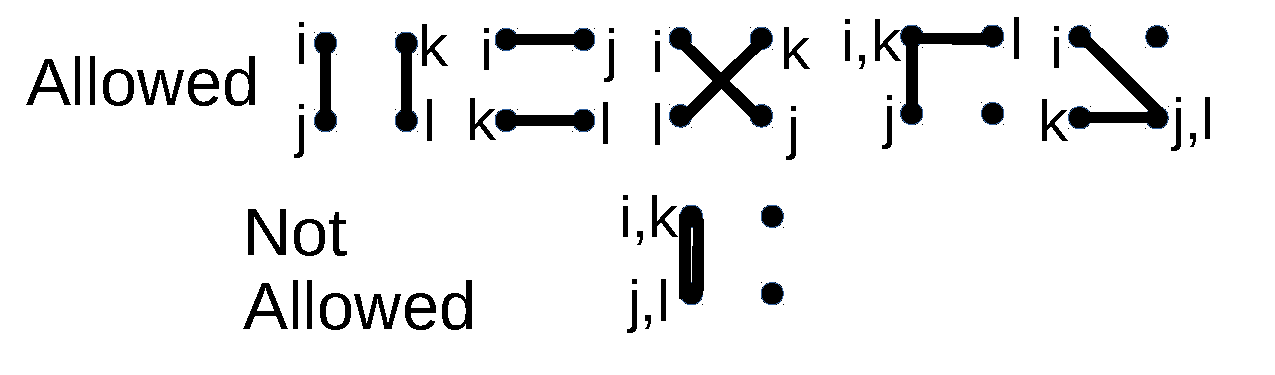
\includegraphics[width=1.0\textwidth]{figures/pairing_fullquad.pdf}
\end{center}
\end{frame}

\begin{frame}{Improved Trial Wave Function - Quadratic Correlations}
\begin{center}
   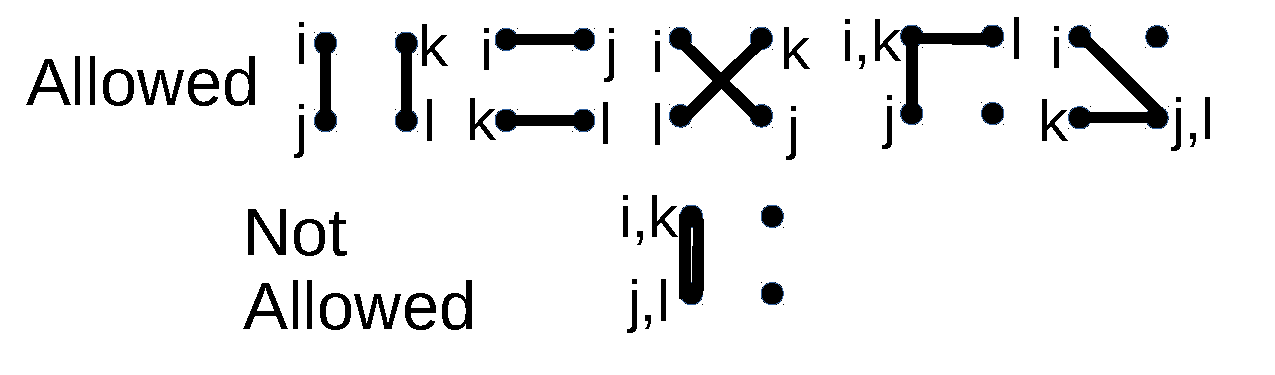
\includegraphics[width=0.6\textwidth]{figures/pairing_fullquad.pdf}
\end{center}
\begin{itemize}
   \item Calculation time can be saved by just looking at {\bf independent pairs} since they capture most of the physics.
\end{itemize}
\uncover<2>{
\begin{equation*}
   \Psi_0(\r_1,\ldots,\r_A) = \left[1+\sum\limits_{i<j}\mathcal{O}_{ij}+\sum\limits_{i<j}\sum_{\substack{k<l\\ij \ne kl}}\mathcal{O}_{ij}\mathcal{O}_{kl}\right]\Phi(\r_1,\ldots,\r_A)
\end{equation*}
\begin{center}
   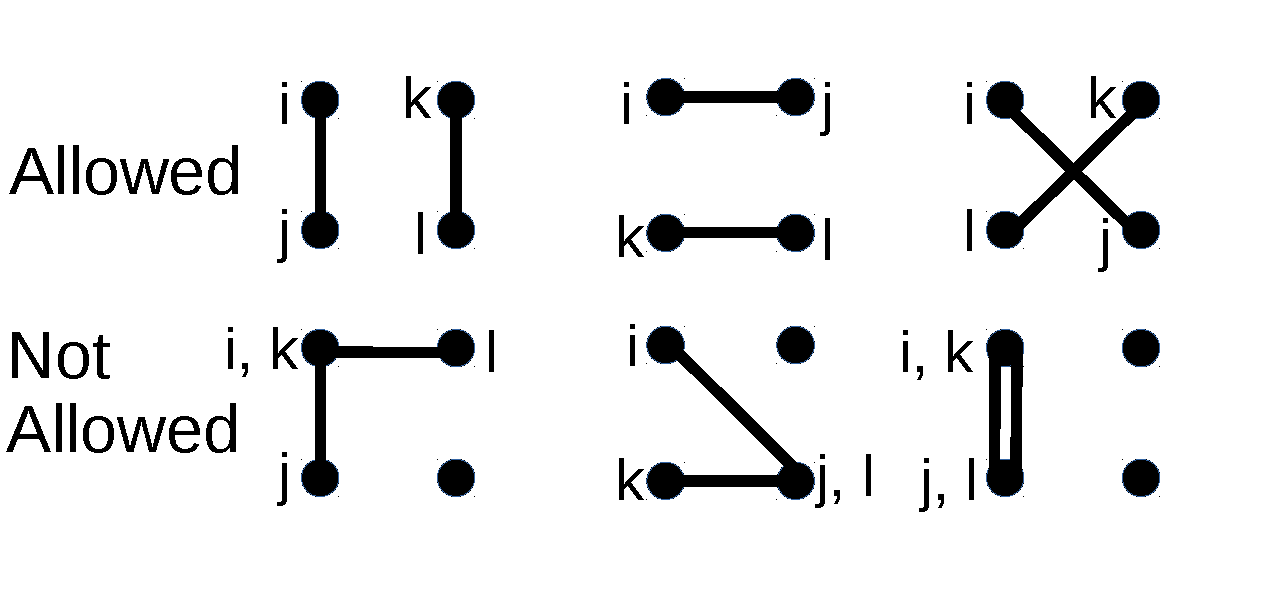
\includegraphics[width=0.6\textwidth]{figures/pairing.pdf}
\end{center}
}
\end{frame}

\begin{frame}{Results}
\begin{textblock*}{\textwidth}(0.0cm,-0.6cm) % {block width} (coords)
\begin{figure}[h]
   \centering
   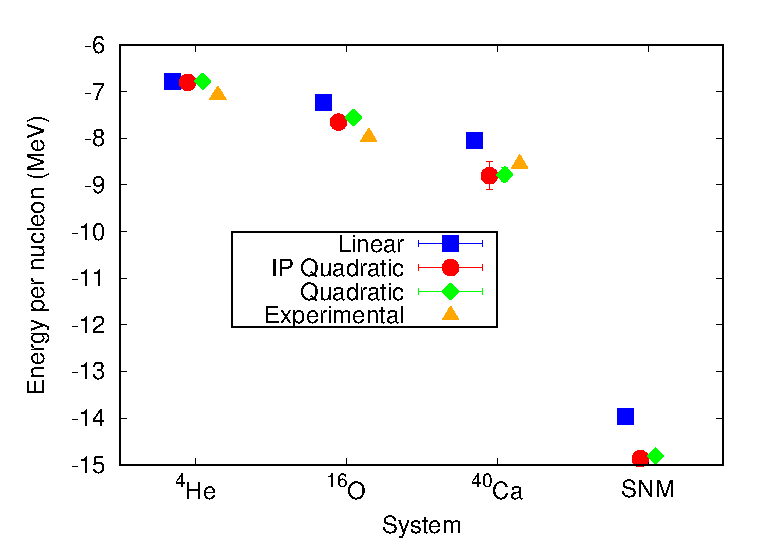
\includegraphics[width=0.7\textwidth]{figures/energy.eps}
\end{figure}
\end{textblock*}
~\\~\\~\\~\\~\\~\\~\\~\\
~\\~\\
\tiny
\begin{table}[htb]
\centering
\caption[]{Energy (*per nucleon) in MeV}
\begin{tabular}{ccccc}
\hline\hline
System & Linear & IP Quadratic & Quadratic & Experimental\\
\hline
${}^{4}${He}   & -27.14(4) & -27.19(3)    & -27.11(3)    & -28.296   \\
${}^{16}${O}   & -115.7(9) & -122.4(1.5)  & -120.8(1.3)  & -127.62   \\
${}^{40}${Ca}  & -322(3)   & -350(10)     & -351(6)      & -342.1    \\
SNM*           & -13.97(3) & -14.87(4)    & -14.81(3)    &           \\
\hline\hline
\end{tabular}
\label{tab:psi2}
\end{table}
{\tiny D. Lonardoni et al. \textit{Phys. Rev. C.,} \textbf{97}, 044318, 2018.}
\end{frame}

\begin{frame}{Quadratic Correlation Cost}
\begin{figure}[h]
   \centering
   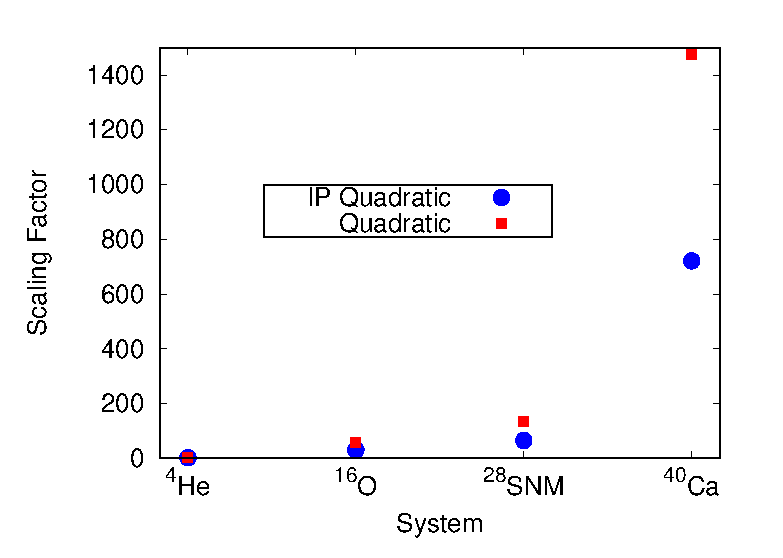
\includegraphics[width=0.65\textwidth]{figures/scaling.eps}
\end{figure}
\vspace{-0.2cm}
\begin{table}[h!]
   \centering
   \begin{tabular}{ccccc}
      \hline \hline
       & $^{4}$He & $^{16}$O & SNM(28) & $^{40}$Ca \\
      \hline
      IP Quadratic & 1.73 & 30.7 & 64.8 & 720.9 \\
      Quadratic & 2.00 & 58.8 & 133.6 & 1473.9 \\
      \hline \hline
   \end{tabular}
\end{table}
\end{frame}

\begin{frame}{Neutron Stars - Preliminary}
\begin{itemize}
   \item Use new wave function to study $\alpha$ formation in the inner crust of neutron stars.
   \begin{equation*}
      E_\alpha = E_\text{Nn+2p} - E_\text{(N-2)n}
   \end{equation*}
\end{itemize}
\vspace{-0.5cm}
\begin{figure}[h]
   \centering
   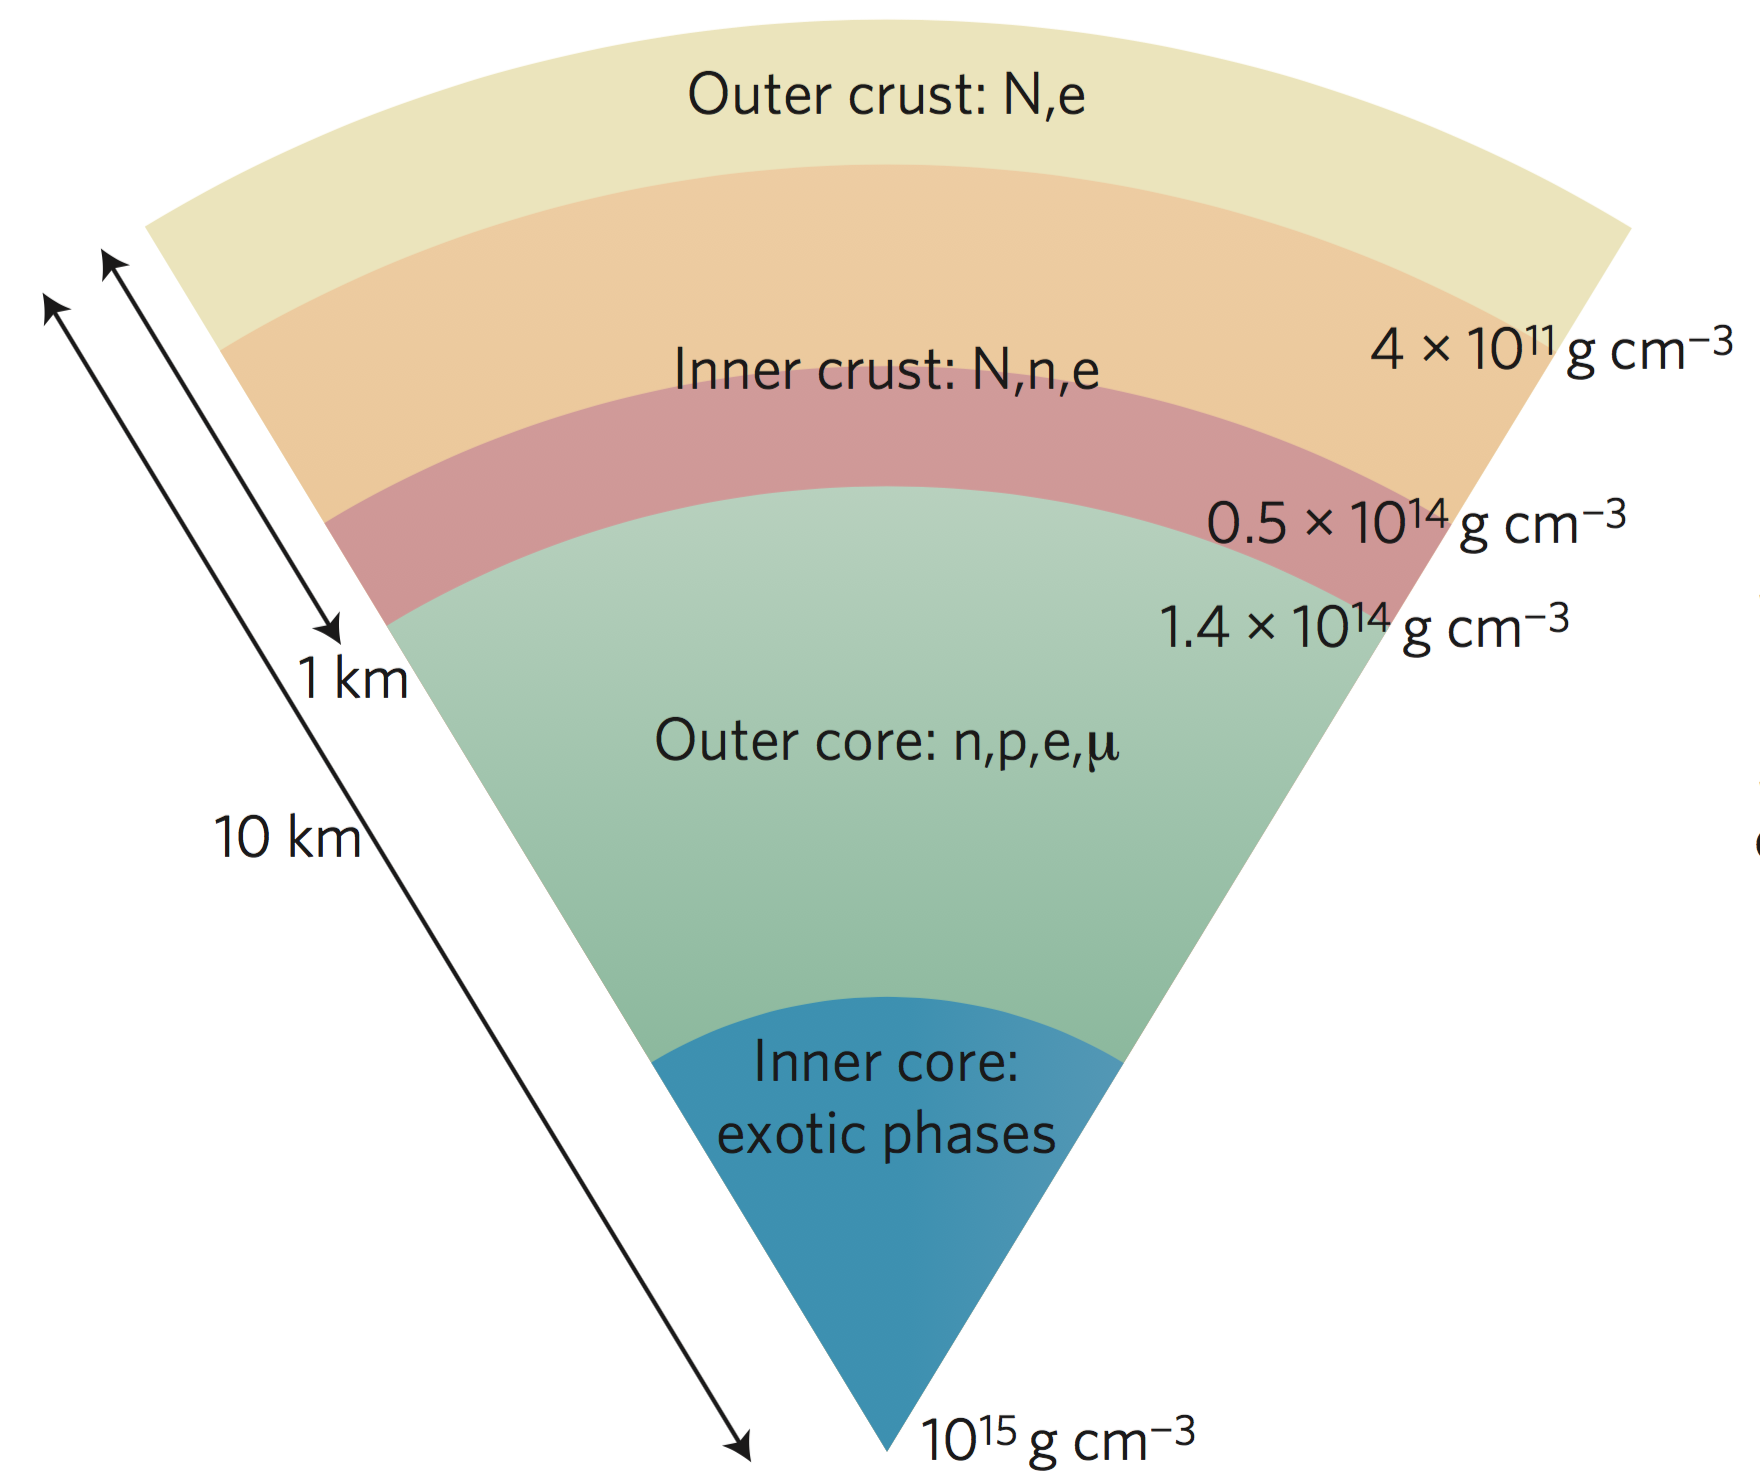
\includegraphics[width=0.5\textwidth]{figures/neutronstar.png}
\end{figure}
{\tiny W. Newton {\it Nature Physics} {\bf 9}, 396-397 (2013)}
%\begin{textblock*}{\textwidth}(8.1cm,-4.6cm) % {block width} (coords)
\begin{textblock*}{\textwidth}(8.1cm,-4.4cm) % {block width} (coords)
   \tiny $\approx$ 0.00024 fm$^{-3}$
\end{textblock*}
%\begin{textblock*}{\textwidth}(7.8cm,-4.1cm) % {block width} (coords)
\begin{textblock*}{\textwidth}(7.8cm,-3.9cm) % {block width} (coords)
   \tiny $\approx$ 0.030 fm$^{-3}$
\end{textblock*}
%\begin{textblock*}{\textwidth}(7.6cm,-3.8cm) % {block width} (coords)
\begin{textblock*}{\textwidth}(7.6cm,-3.6cm) % {block width} (coords)
   \tiny $\approx$ 0.084 fm$^{-3}$
\end{textblock*}
%\begin{textblock*}{\textwidth}(6.4cm,-1.3cm) % {block width} (coords)
\begin{textblock*}{\textwidth}(6.4cm,-1.1cm) % {block width} (coords)
   \tiny $\approx$ 0.60 fm$^{-3}$
\end{textblock*}
\end{frame}

\begin{frame}{\large Alpha Particle Clustering in Mostly Neutron Matter - Preliminary}
\begin{itemize}
   \item If alpha particles form in nearly neutron matter then we should be able to estimate their energy by
   \begin{equation*}
      E_\alpha = E_\text{14n+2p} - E_\text{12n}
   \end{equation*}
   \vspace{-0.25cm}
   \begin{columns}
   \begin{column}{0.6\textwidth}
   \begin{figure}[h]
      \centering
      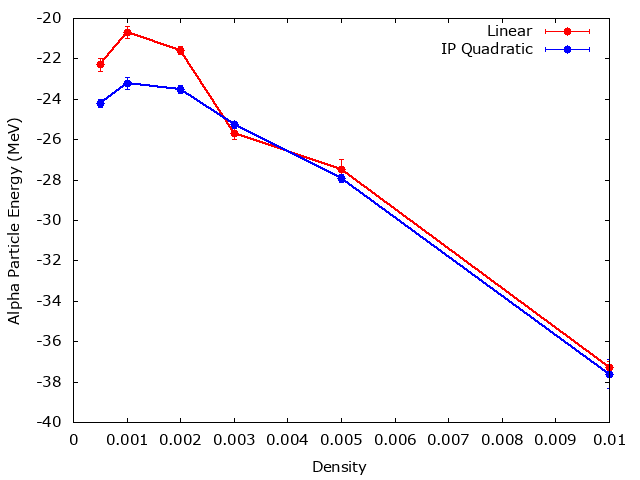
\includegraphics[width=\textwidth]{figures/alpha.png}
   \end{figure}
   \end{column}
   \hspace{-0.6cm}
   \begin{column}{0.4\textwidth}
   \begin{table}[h!]
      \footnotesize
      \centering
      \caption{Alpha energy in MeV}
      \begin{tabular}{ccc}
         \hline \hline
         $\rho$ (fm$^{-3}$) & lin & ip \\
         \hline
         0.00025  & -23.5(5)  & -25.4(2)  \\
         0.0005   & -22.3(3)  & -24.2(2)  \\  
         0.001    & -20.7(3)  & -23.2(3)  \\  
         0.002    & -21.6(2)  & -23.5(3)  \\  
         0.003    & -25.7(3)  & -25.26(18)\\
         0.005    & -27.5(5)  & -27.9(2)  \\  
         0.01     & -37.3(3)  & -37.6(7)  \\  
         \hline \hline
      \end{tabular}
   \end{table}
   \end{column}
   \hspace{0.6cm}
   \end{columns}
\end{itemize}
\end{frame}

\begin{frame}{Pair Correlation Function - Preliminary}
\vspace{-0.1cm}
\begin{equation*}
   g_{pp}(r) = \frac{1}{4\pi r^2} \bra{\Psi}\sum\limits_{i<j}\hat{p}_i\hat{p}_j\delta(r-r_{ij})\ket{\Psi}
\end{equation*}
\vspace{-0.4cm}
\begin{figure}[h]
   \centering
   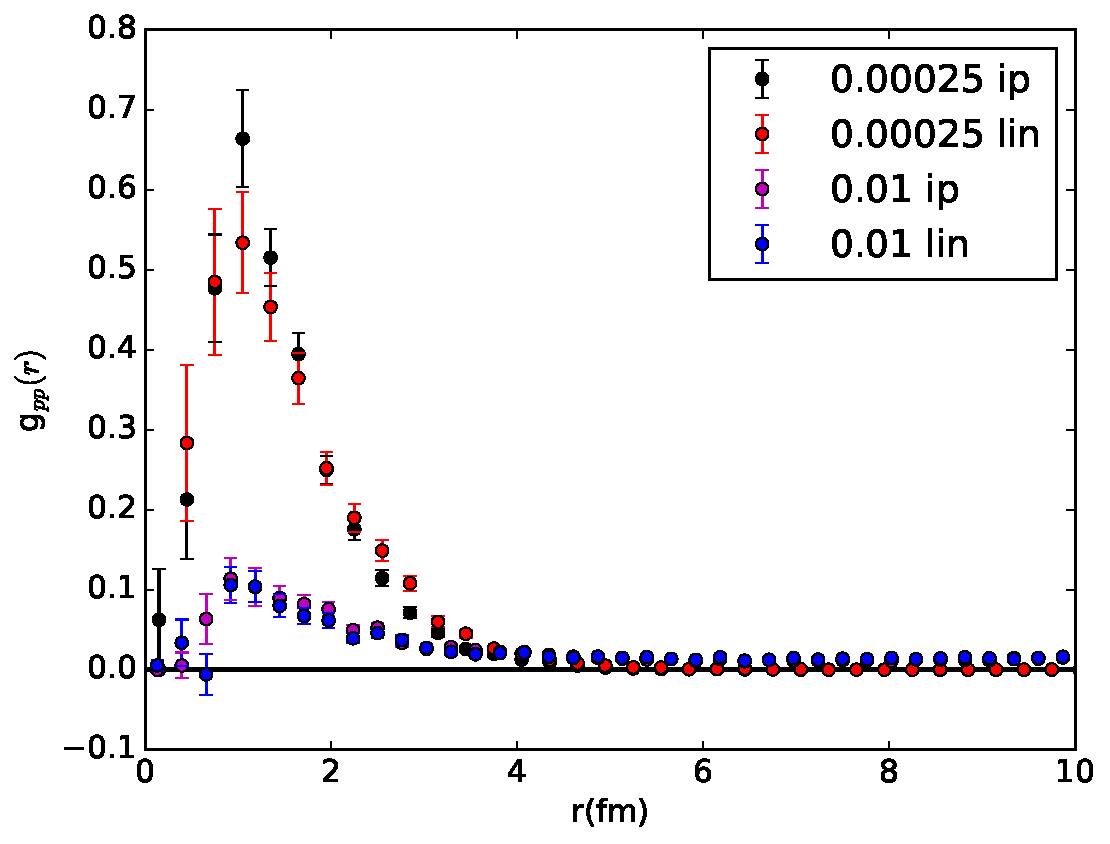
\includegraphics[width=0.80\textwidth]{figures/gpp.pdf}
\end{figure}
\end{frame}

\begin{frame}{Pair Correlation Function - Preliminary}
\vspace{-0.1cm}
\begin{equation*}
   g_{pp}(r) = \frac{1}{4\pi r^2} \bra{\Psi}\sum\limits_{i<j}\hat{p}_i\hat{p}_j\delta(r-r_{ij})\ket{\Psi}
\end{equation*}
\vspace{-0.4cm}
\begin{figure}[h]
   \centering
   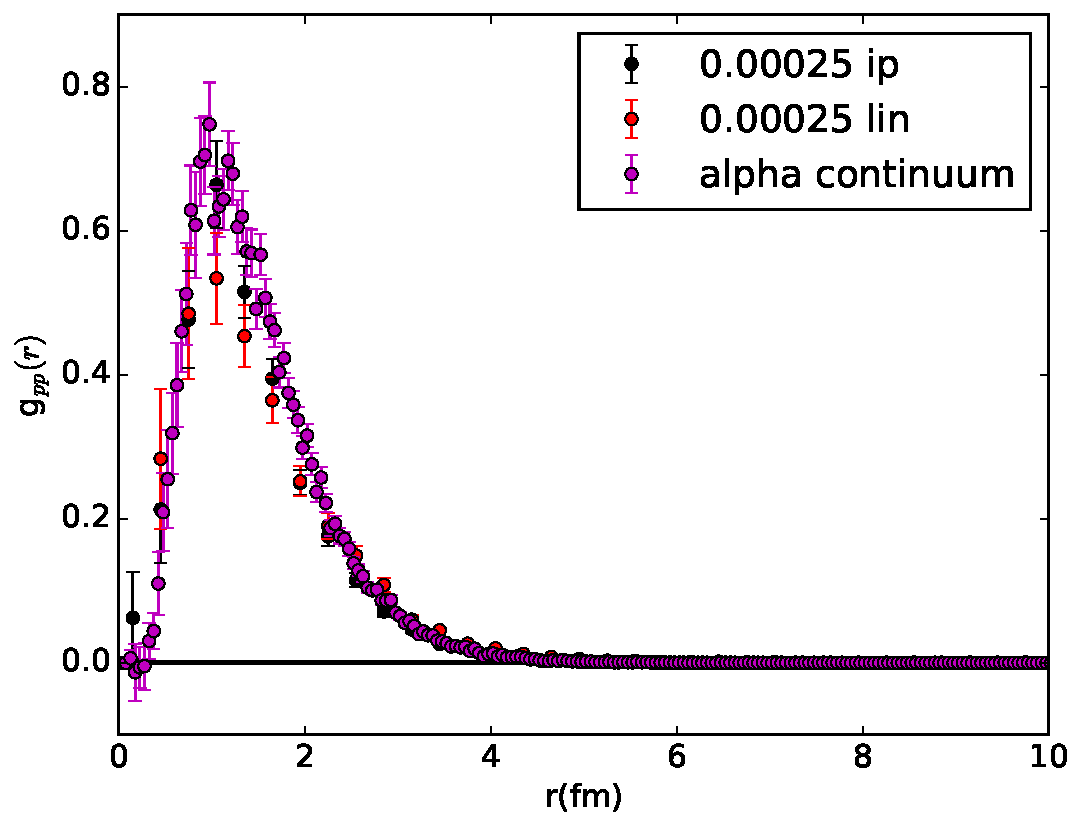
\includegraphics[width=0.80\textwidth]{figures/gpp_continuum.pdf}
\end{figure}
\end{frame}

\begin{frame}{Future Work}
\begin{itemize}
   \item Other improvements to trial wave function
   \item Neutron star equation of state, $E(\rho)$
   \begin{itemize}
      \item Using $\chi$EFT interaction
      \item Understanding the hyperon problem
   \end{itemize}
   \item Understand what is happening at higher nuclear densities
   \item Other interesting projects that push our understanding and application of nuclear physics
   \item Any interesting physics, especially with applications to computation
\end{itemize}
\end{frame}

\begin{frame}{Future Work - Neutron Stars}
\begin{center}
   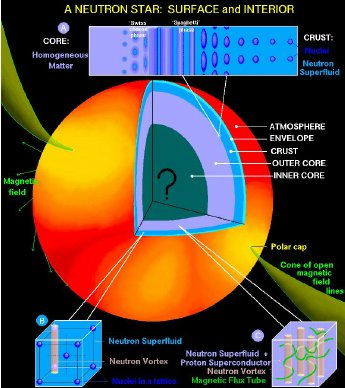
\includegraphics[height=0.7\textwidth]{figures/neutron_star.jpg}
\end{center}
\end{frame}

\begin{frame}{Future Work - Hyperon Problem}
\begin{center}
   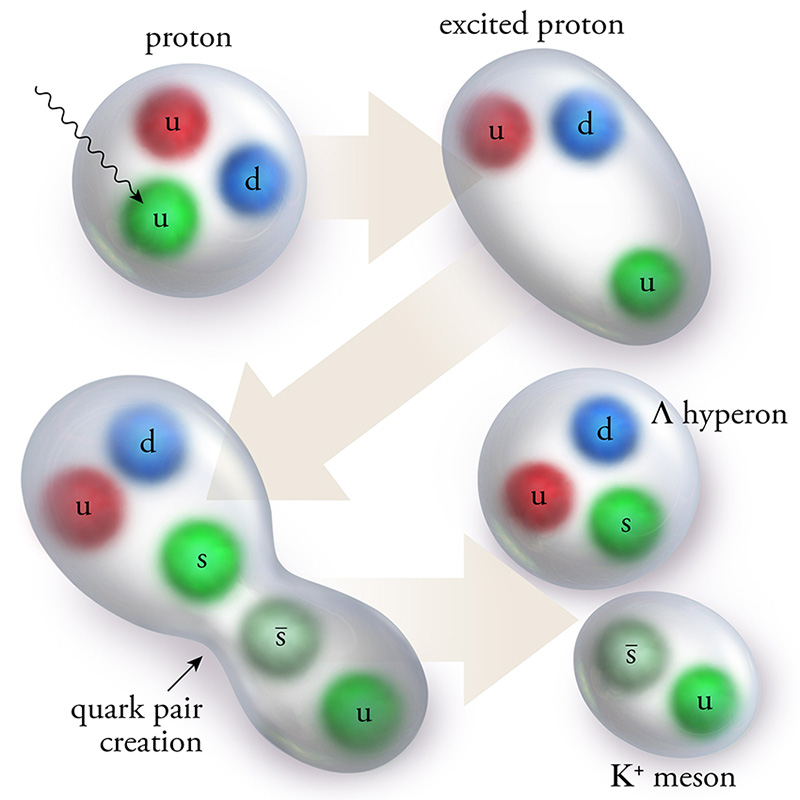
\includegraphics[width=0.3\textwidth]{figures/lambda.jpg}
   ~\\
   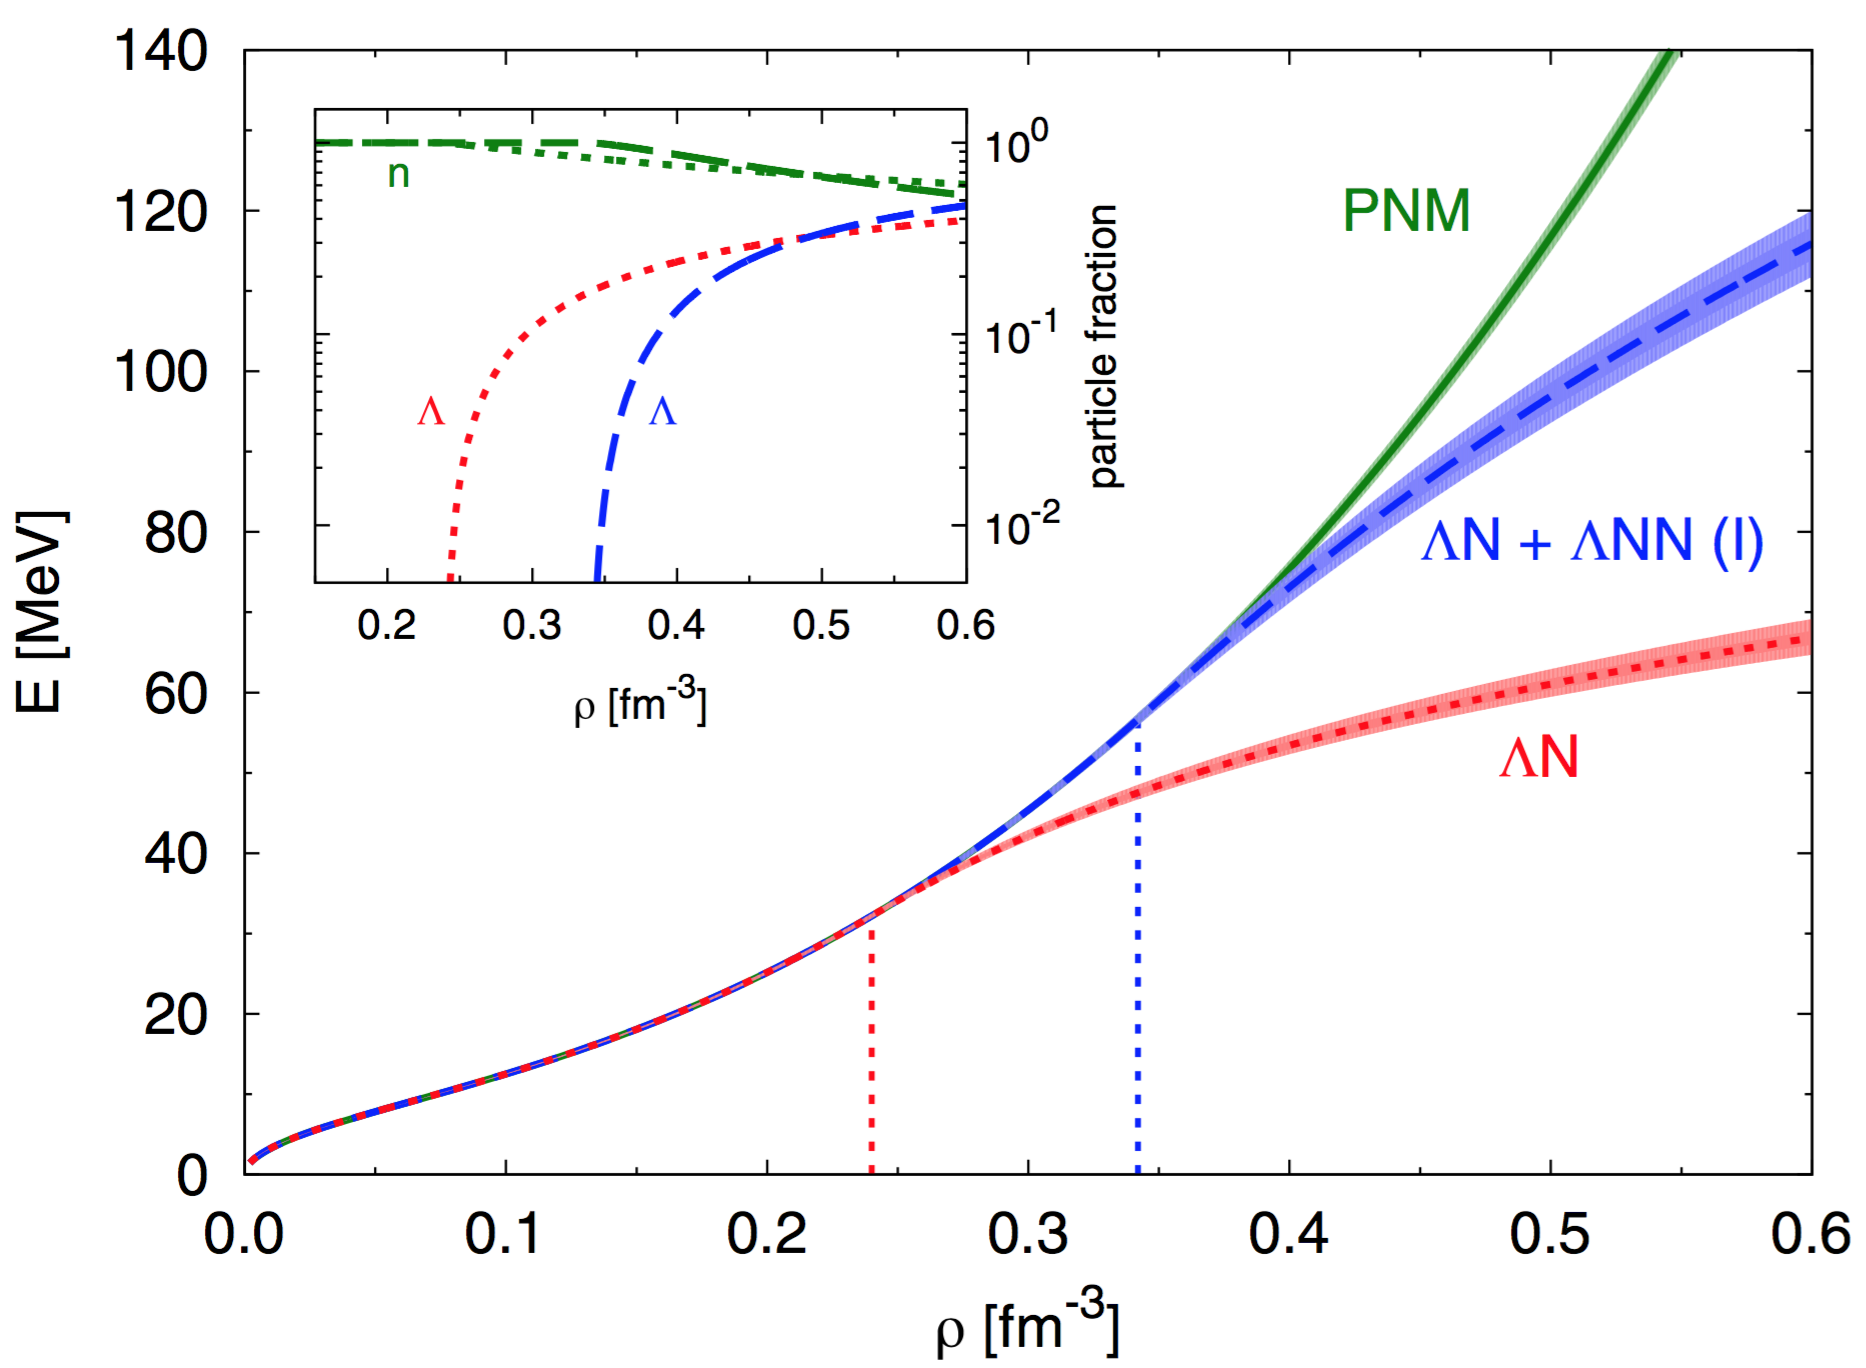
\includegraphics[width=0.5\textwidth]{figures/ns_eos.png}
   ~
   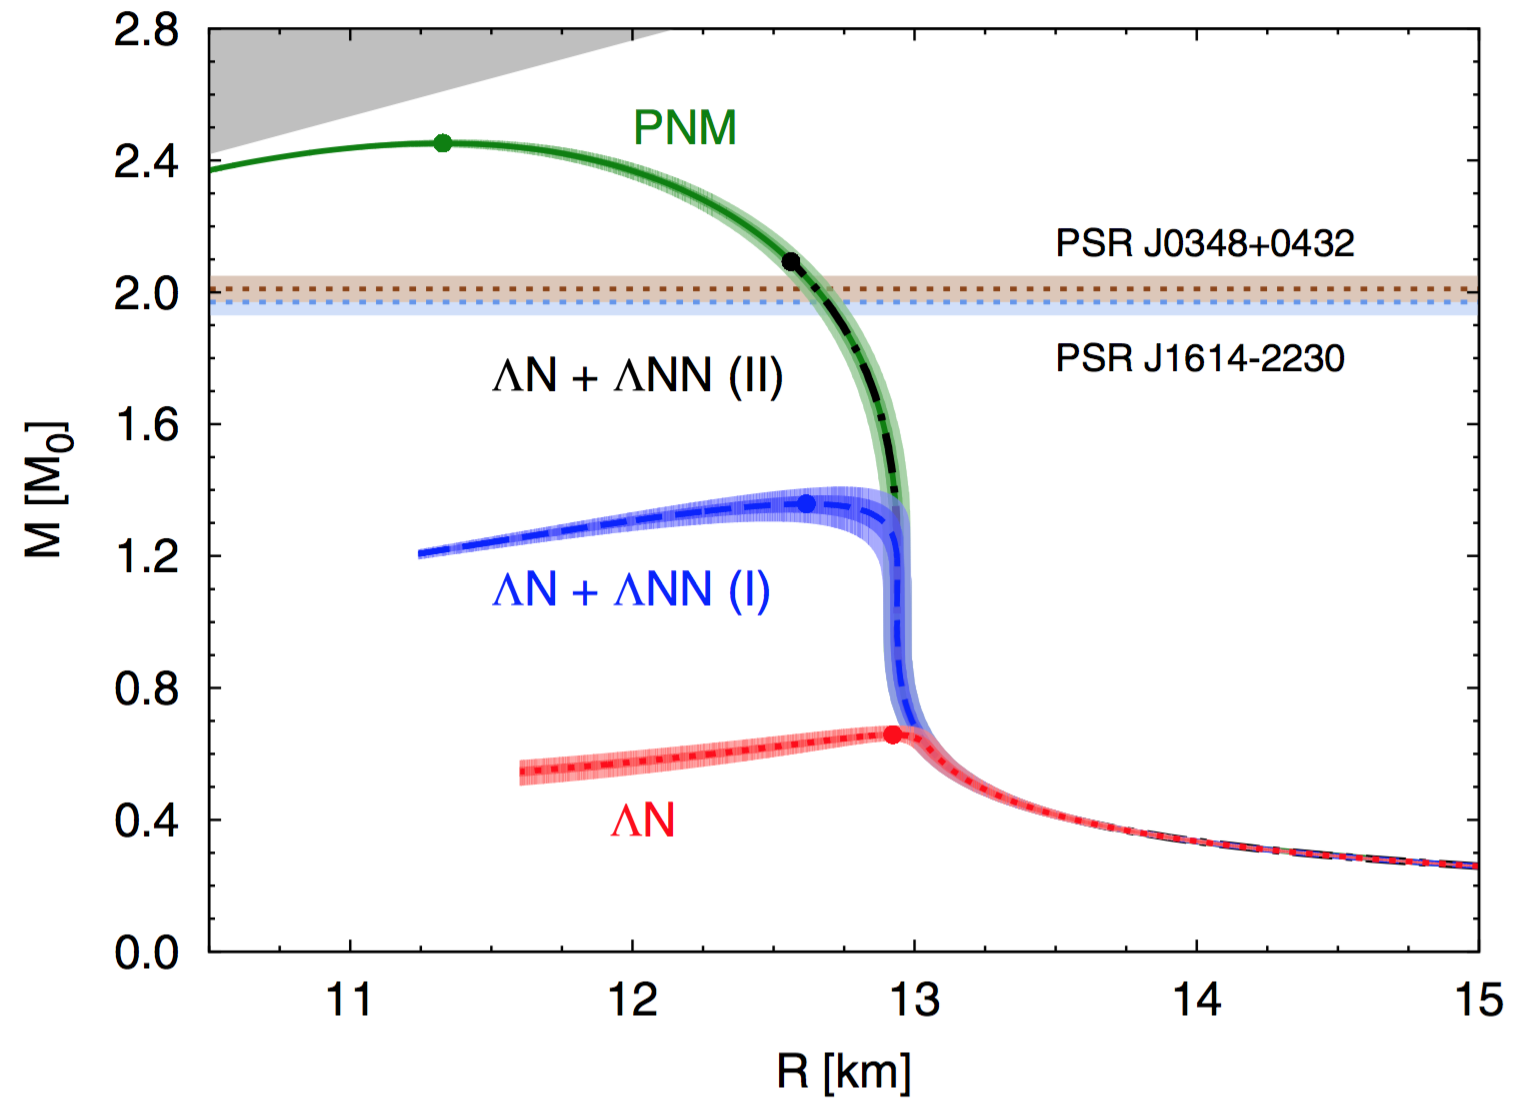
\includegraphics[width=0.5\textwidth]{figures/mr.png}
\end{center}
{\tiny Diego Lonardoni et al. \textit{Phys. Rev. Lett.,} \textbf{114}, 092301, 2015.}
\end{frame}

\begin{frame}{Conclusion/Summary}
\begin{itemize}
   \item Quantum Monte Carlo is a powerful method for studying nuclear systems.
   \item We need to improve the wave function to study larger, more interesting systems.
   \item There are a variety of interesting problems that would be fun to do in collaboration with SUU students and faculty.
\end{itemize}
\end{frame}

\begin{frame}{Thanks}
PhD Advisor: Kevin Schmidt (ASU) \\
Collaborators: Stefano Gandolfi (LANL) and Joe Carlson (LANL)
\\~\\
\begin{figure}[h]
   \centering
   
\includegraphics[width=0.30\textwidth]{figures/asu_university_vert_rgb_maroongold_150.png}
   
\includegraphics[width=0.36\textwidth]{figures/xsede-full-color.jpg}
   
\includegraphics[width=0.30\textwidth]{figures/NSF_4-Color_bitmap_Logo.png}
\end{figure}
\end{frame}

\begin{frame}{Picture References}
\tiny
Questions comic, accessed 2 Mar 2019: \href{https://socializingsciencevu.com/category/tips-tricks/}{https://socializingsciencevu.com/category/tips-tricks/}
Atomic model, accessed 1 Mar 2019: \href{http://www.whoinventedfirst.com/who-discovered-the-atom/}{http://www.whoinventedfirst.com/who-discovered-the-atom/}\\
Nuclear power plant, accessed 1 Mar 2019: \href{https://phys.org/news/2016-11-future-nuclear-energy.html}{https://phys.org/news/2016-11-future-nuclear-energy.html}\\
Radiotherapy, accessed 1 Mar 2019: \href{https://www.bupa.co.uk/health-information/cancer/radiotherapy}{https://www.bupa.co.uk/health-information/cancer/radiotherapy}\\
MRI, accessed 1 Mar 2019: \href{https://www.123rf.com/photo_20891118_mri-scan-of-the-human-brain.html}{https://www.123rf.com/photo\_20891118\_mri-scan-of-the-human-brain.html}
Mummy, accessed 1 Mar 2019: \href{https://www.smithsonianmag.com/science-nature/carbon-dating-crucial-scientific-technique-jeopardy-thanks-our-pollution-heres-easy-way-fix-it-180961345/}{https://www.smithsonianmag.com/science-nature/carbon-dating-crucial-scientific-technique-jeopardy-thanks-our-pollution-heres-easy-way-fix-it-180961345/}\\
Electron Orbitals, accessed 2 Mar 2019: \href{https://en.wikipedia.org/wiki/Atomic_orbital}{https://en.wikipedia.org/wiki/Atomic\_orbital}\\
LHC, accessed 2 Mar 2019: \href{https://www.scientificamerican.com/article/proton-smashing-resumes-at-the-world-s-largest-particle-accelerator/}{https://www.scientificamerican.com/article/proton-smashing-resumes-at-the-world-s-largest-particle-accelerator/}\\
Pion exchange feynman diagram, accessed 2 Mar 2019: \href{https://ati.tuwien.ac.at/research_areas/nuclear_and_particle_physics/research/fundamental_interactions/strong_interaction/EN/}{https://ati.tuwien.ac.at/research\_areas/nuclear\_and\_particle\_physics/research/fundamental\_interactions/strong\_interaction/EN/}\\
Riemann sum, accessed 2 Mar 2019: \href{https://en.wikipedia.org/wiki/Riemann\_sum\#/media/File:Riemann\_sum\_convergence.png}{https://en.wikipedia.org/wiki/Riemann\_sum\#/media/File:Riemann\_sum\_convergence.png}\\
Neutron star, accessed 4 Mar 2019: \href{https://www.researchgate.net/publication/23952027_Nuclear_Physics_of_Neutron_Stars/figures}{https://www.researchgate.net/publication/23952027\_Nuclear\_Physics\_of\_Neutron\_Stars/figures}\\
Lambda hyperon formation, accessed 4 Mar 2019: \href{https://science.energy.gov/np/highlights/2015/np-2015-08-b/}{https://science.energy.gov/np/highlights/2015/np-2015-08-b/}\\
\end{frame}

\iffalse
\appendix
\begin{frame}{Variational Monte Carlo - Implementation}
\begin{enumerate}
   \item Generate N configurations (walkers) distributed randomly.
   \item Loop over each walker and do the following
   \begin{enumerate}
      \setlength\itemsep{0.2em}
      \item Calculate $P(\R) = \left|\braket{\Psi_T}{\R}\right|^2$.
      \item Propose a move $\R' = \R + \Delta\xi$, where $\xi$ could be a vector of random variables from a Gaussian.
      \item Calculate $P(\R') = \left|\braket{\Psi_T}{\R'}\right|^2$.
      \item Calculate the probability of acceptance $A=\mathrm{min}\left(1,\frac{P(\R')}{P(\R)}\right)$.
      \item If accepted then $\R \rightarrow \R'$, else the next position in the Markov Chain for that walker is the same as the last, namely $\R$.
   \end{enumerate}
   \item Calculate observables and repeat steps 2 until energy is minimized or uncertainties are low enough.
\end{enumerate}
\end{frame}

\begin{frame}{Diffusion Monte Carlo - Branching}
Branching: Each walker can be deleted or multiply. The number of walkers that continues is equal to $\mathrm{int}\left(w(\R')+\xi\right)$, where $\xi$ is a uniform random number from $[0,1]$.
\begin{columns}
\begin{column}{0.4\textwidth}
\begin{figure}
   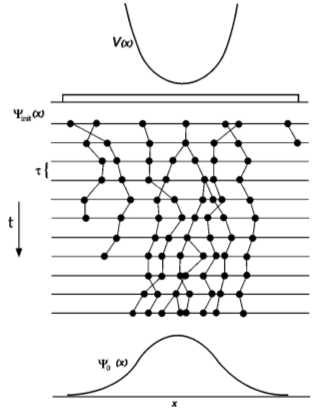
\includegraphics[width=0.9\textwidth]{figures/branch_full.png}
\end{figure}
\end{column}
\begin{column}{0.7\textwidth}
   {\color{blue}{Figure:}} Reprinted from W.M.C. Foulkes et al. \textit{Rev. Mod. Phys.,} 73:33-83, 2001.
\end{column}
\end{columns}
\end{frame}

\begin{frame}{Diffusion Monte Carlo - Implementation}
\begin{enumerate}
   \item Start with N configurations (walkers) from VMC
   \item Loop over each walker and do the following
   \begin{enumerate}
      \setlength\itemsep{0.2em}
      \item Propose a move, $\R' = \R + \chi$, where $\chi$ is a vector of random numbers from the shifted Gaussian $\exp\left(\frac{m}{2\hbar^2\Delta\tau}\left(\R'-\R+2\frac{\nabla\Psi_I(\R')}{\Psi_I(\R')}\right)^2\right)$.
      \item The move is then accepted with the probability $A(\R'\leftarrow\R)=\mathrm{min}\left(1,\frac{\Psi_T^2(\R')}{\Psi_T^2(\R)}\right)$.
      \item Calculate the weight $w(\R')=\exp\left(-\left(E_L(\R')+E_L(\R)-2E_0\right)\Delta\tau/2\right)$.
      \item Do branching.
      \item Calculate and collect the observables and uncertainties needed and increase the imaginary time by $\Delta\tau$.
   \end{enumerate}
   \item Repeat from step 2 to 6 until the uncertainties are small enough.
\end{enumerate}
\end{frame}
\fi

\end{document}
